\documentclass[a4paper, 10pt, final, garamond]{book}
\usepackage{cours-preambule}

\titleformat{\item}{}{\arabic{item})}{.5em}{}{}
\titleformat{\subitem}{}{\arabic{item}) \alph{subitem} --}{.5em}
{}{}

\makeatletter
\renewcommand{\@chapapp}{Devoir maison -- num\'ero}
\makeatother

\begin{document}
\setcounter{chapter}{4}

\chapter{Commentaires sur le DM n\degree5}

\begin{NCprop}[width=\linewidth]{\centering\bfseries\ Rappel des malus}
    Chacune des lettres suivantes sur vos copies sont des malus de \num{1}
    point.\smallbreak
    \begin{minipage}{0.50\linewidth}
        \begin{itemize}
            \item A~: application numérique mal faite~;
            \item C~: copie grand carreaux~;
        \end{itemize}
    \end{minipage}
    \begin{minipage}{0.50\linewidth}
        \begin{itemize}
            \item H~: homogénéité non respectée~;
        \end{itemize}
    \end{minipage}
\end{NCprop}

\begin{enumerate}
    \item RAS.
      \hfill \textcolor{ForestGreen}{/2}
    \item Attention aux définitions~:
      \[
              \begin{aligned}
              [C_V] &= \si{J.K^{-1}}
                    &
              \Ra
                    &
              \qquad
              U_{\rm GP} = C_V T
              \\
              \left[\frac{C_V}{n}\right] = [C_{V,m}] &= \si{J.K^{-1}.mol^{-1}}
                    &
              \Ra
                    &
              \qquad
              U_{\rm GP} = nC_{V,m} T
              \\
              \left[\frac{C_V}{m}\right] = [c_V] &= \si{J.K^{-1}.kg^{-1}}
                    &
              \Ra
                    &
              \qquad
              U_{\rm GP} = mc_V T
            \end{aligned}
      \]
      \hfill \textcolor{ForestGreen}{/3}
    \item RAS (soyez exhaustif-ves dans vos réponses)
      \hfill \textcolor{ForestGreen}{/4}
    \item \textbf{Point pour le schéma/traduction de la transformation.}.
      Attention cependant,
      \begin{center}
          \huge
          Mécaniquement réversible n'est pas automatiquement réversible~!!
          Mécaniquement réversible $\Ra P_{\rm ext} = P$.
      \end{center}
      Mécaniquement réversible + monotherme $\equiv$ QS $\Ra$ isotherme.
      \textbf{Justifiez $T_1' = T_1$}.
      \hfill \textcolor{ForestGreen}{/4}
    \item Faites le calcul ! Attention, {\Large $P \neq P_1$}. Donnez la
      définition de base de $W = -\int^{V_i}_{V_f}P_{\rm ext}\dd{V}$.
      \hfill \textcolor{ForestGreen}{/5}
    \item Énoncez soit la loi de \textsc{Joule}, soit directement $\Delta{U} =
      C_V \Delta{T}$.
      \hfill \textcolor{ForestGreen}{/4}
    \item RAS.
      \hfill \textcolor{ForestGreen}{/1}
    \item Beaucoup de points perdus ici~: encore une fois, \textbf{mécaniquement
      réversible $\nRightarrow$ réversible}. Il fallait \textbf{calculer
      $\Delta{S}$ et trouver $S_c = 0$}.
    \item \textbf{Point pour le schéma/traduction de la transformation.} Système
      isolé $\Ra \Delta{U} = 0$. Non, l'évolution du gaz n'est \textbf{pas
      isochore} (le volume change). Non, on ne peut pas supposer la
      transformation comme étant quasi-statique.
      \hfill \textcolor{ForestGreen}{/4}
    \item RAS.
      \hfill \textcolor{ForestGreen}{/1}
    \item RAS.
      \hfill \textcolor{ForestGreen}{/1}
    \item Justifier l'irréversibilité (gradient de pression).
      \hfill \textcolor{ForestGreen}{/2}
\end{enumerate}

\begin{center}
    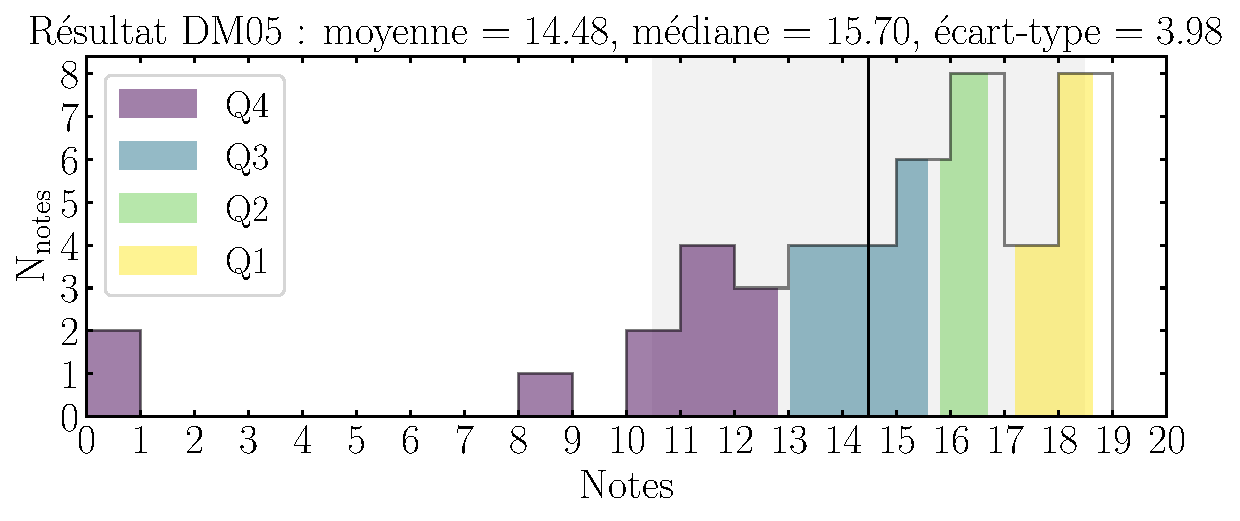
\includegraphics[width=.8\linewidth]{res_DM05.pdf}
\end{center}

\end{document}
